\documentclass{article}

% ICML 2026 style — replace with target venue style file before submission
\usepackage[preprint]{neurips_2025}

\usepackage[utf8]{inputenc}
\usepackage[T1]{fontenc}
\usepackage{hyperref}
\usepackage{url}
\usepackage{booktabs}
\usepackage{amsfonts}
\usepackage{nicefrac}
\usepackage{microtype}
\usepackage{xcolor}
\usepackage{graphicx}
\usepackage{subcaption}
\usepackage{multirow}
\usepackage{amsmath}
\usepackage{xspace}

% Convenience macros
\newcommand{\method}{HateLens}
\newcommand{\eg}{e.g.,\xspace}
\newcommand{\ie}{i.e.,\xspace}
\newcommand{\etal}{\textit{et al.}\xspace}
\newcommand{\tl}{TinyLlama\xspace}
\newcommand{\todo}[1]{\textcolor{red}{[TODO: #1]}}

% ─────────────────────────────────────────────────────────────────────────────
\title{Beyond Binary Labels: Structured Multi-Task Supervision Improves\\
Robustness of Lightweight Hate Speech Detection}

% Anonymous for blind review — fill in before camera-ready
\author{%
  Anonymous
}

\begin{document}
\maketitle

% ─────────────────────────────────────────────────────────────────────────────
\begin{abstract}
We propose \method{}, a structured multi-task learning framework that extends
parameter-efficient fine-tuning (PEFT) of small decoder language models for
hate speech detection beyond binary classification.
Building on \citet{sen2024hatetinyllm}, who demonstrated that LoRA-tuned
TinyLlama-1.1B achieves competitive binary accuracy on DynaHate and HateEval,
we ask whether jointly predicting auxiliary attributes—hate type, target group,
and explicitness—together with optional rationale-token supervision and
pair-consistency regularization, improves out-of-distribution robustness.
We train on DynaHate (41k entries) with optional HateXplain joint data and
evaluate on three benchmarks: in-domain test splits, cross-benchmark transfer
to HateEval, and functional robustness via HateCheck (3,728 structured test cases).
Our structured model raises HateCheck F1 from 0.815 to 0.921 ($+10.6$ pp),
in-domain DynaHate F1 from 0.710 to 0.815 ($+10.5$ pp), and cross-benchmark
HateEval F1 from 0.603 to 0.615—all with only 780K trainable parameters.
Ablations show that auxiliary objective supervision is the primary driver
of functional robustness; pair-consistency regularization further improves
cross-benchmark transfer.
A controlled PEFT comparison confirms that LoRA, QLoRA, and DoRA reach
within 1 pp of each other on HateCheck (F1 0.878, 0.870, 0.880), validating
parameter-efficient training for deployment.
Code and data loaders are publicly available.\footnote{\url{https://github.com/EmaRimoldi/HateLens}}
\end{abstract}

% ─────────────────────────────────────────────────────────────────────────────
\section{Introduction}
\label{sec:intro}

Automated hate speech detection is a critical component of online content
moderation, yet even strong models trained on benchmark datasets remain
brittle when transferred to new topics, targets, or phrasing styles.
A recurring finding across evaluations is that high held-out accuracy does not
guarantee robustness on the edge cases that matter most in deployment: denial
of hate (\textit{"I'm just joking"}), references involving reclaimed slurs, or
compositional rephrasing that preserves hateful intent while evading keyword
filters \citep{rottger2021hatecheck}.

\paragraph{The gap in existing work.}
\citet{sen2024hatetinyllm} showed that LoRA fine-tuning of small decoder language
models (TinyLlama, Phi-2, OPT-1.3B) achieves over 80\% accuracy on DynaHate
\citep{vidgen2021dynahate} and HateEval \citep{basile2019semeval}—competitive with
models ten times larger.
Their work, however, focused exclusively on binary classification: is a post
hateful or not?
Binary supervision provides no signal about \emph{why} a model should classify
a post as hateful, nor about the \emph{type} or \emph{target} of the hate.
This absence of auxiliary structure leaves two problems unaddressed:
(1) models that learn surface features instead of semantic content fail on
adversarially generated cases that HateCheck targets, and
(2) models trained on a single dataset transfer poorly to out-of-distribution
benchmarks even when overall accuracy remains high.

\paragraph{Our approach.}
We extend TinyLlama+LoRA with \emph{structured multi-task supervision}: a shared
PEFT backbone is joined by lightweight heads that predict the primary hate label,
the hate type (e.g., derogation, animosity, dehumanization), the target group
(e.g., race, gender), and the explicitness of expression.
When HateXplain rationale annotations are available, we add token-level rationale
supervision \citep{mathew2021hatexplain}.
When DynaHate pair metadata is available, we apply pair-consistency regularization
that encourages logically entailed pairs to receive consistent predictions.
The backbone remains frozen except for LoRA adapters on the key/value projections,
keeping the total number of trainable parameters at 780K.

\paragraph{Contributions.}
\begin{itemize}
  \item We demonstrate that structured multi-task supervision with lightweight auxiliary
    heads improves HateCheck functional robustness by $+10.6$ pp (F1: 0.815 → 0.921)
    over a well-matched binary baseline using identical PEFT configuration.
  \item We show that joint training with HateXplain provides additional robustness
    gains ($+0.8$ pp HateCheck F1) while preserving in-domain performance.
  \item We present ablation studies revealing that auxiliary-objective supervision
    is the primary driver of robustness, with pair-consistency regularization
    further improving cross-benchmark transfer ($+2.1$ pp HateEval F1 over the
    standard structured model).
  \item We report a controlled PEFT variant comparison (LoRA, QLoRA, DoRA) showing
    near-identical HateCheck performance ($\leq 1$ pp spread), validating the
    choice of lightweight adapters for deployment.
  \item We release \method{}, an open codebase with reproducible training pipelines,
    unified evaluation, calibration metrics (ECE, Brier score), and all data loaders.
\end{itemize}

% ─────────────────────────────────────────────────────────────────────────────
\section{Related Work}
\label{sec:related}

\paragraph{Hate speech detection with PLMs.}
BERT-based encoders established strong baselines for automated hate detection
\citep{basile2019semeval,vidgen2021dynahate}.
\citet{rottger2021hatecheck} introduced HateCheck to expose systematic weaknesses
in these models—including over-sensitivity to identity terms and failure on
negated hate—finding critical errors in all tested systems.
More recent work has shifted toward encoder-only fine-tuning with dataset
unification: \citet{elbahnasawi2025lora} combine LoRA-tuned BERTweet with
rule-based pre-filtering and continuous learning, achieving macro F1 0.85
with only 1.87M trainable parameters on unified datasets.

\paragraph{Tiny decoder LLMs for classification.}
\citet{sen2024hatetinyllm} proposed HateTinyLLM, fine-tuning TinyLlama (1.1B),
Phi-2 (2.7B), and OPT-1.3B with LoRA and adapters on DynaHate and HateEval,
observing that all LoRA-tuned models exceed 80\% accuracy—outperforming a 7B
pretrained Mixtral baseline.
Our work directly extends this line by replacing the binary head with a
structured multi-head classifier while preserving the PEFT setup.

\paragraph{Multi-task hate detection.}
DynaHate includes fine-grained type and target annotations that binary training
ignores \citep{vidgen2021dynahate}.
HateXplain provides rationale spans that ground decisions in textual evidence
\citep{mathew2021hatexplain}.
Multi-task learning over these labels has been explored in shared tasks \citep{prama2025hatesense},
but typically with large encoder or decoder LLMs.
Our work demonstrates that structured multi-task objectives improve robustness
with a 1.1B decoder model and fewer than 1M trainable parameters.

\paragraph{PEFT variants.}
LoRA \citep{hu2022lora} has become the de facto PEFT method for classification.
QLoRA \citep{dettmers2023qlora} extends this with 4-bit quantization for memory
efficiency.
DoRA \citep{liu2024dora} decomposes weight updates into magnitude and direction
components.
Their relative performance on downstream hate detection tasks has not been
systematically compared under controlled conditions; we address this gap.

\paragraph{Calibration and transfer in hate detection.}
Model calibration—the alignment between predicted confidence and true accuracy—
is rarely reported in hate detection benchmarks despite its relevance for
deployment \citep{guo2017calibration}.
Cross-dataset transfer from one hate speech benchmark to another is also
infrequently measured.
We report Expected Calibration Error (ECE) and Brier score alongside standard
classification metrics for all models.

% ─────────────────────────────────────────────────────────────────────────────
\section{Method}
\label{sec:method}

\subsection{Backbone and PEFT}
We use \tl (1.1B parameters, PY007/TinyLlama-1.1B-step-50K-105b) as the
backbone decoder LM.
For binary classification experiments we attach a sequence-classification
head via \texttt{AutoModelForSequenceClassification} (\texttt{task\_type=SEQ\_CLS}).
For structured experiments we use \texttt{task\_type=FEATURE\_EXTRACTION} and
replace the classification head with the multi-head architecture described below.

LoRA adapters are applied to the key ($W_K$) and value ($W_V$) projections in
all self-attention layers with rank $r=8$, scaling factor $\alpha=16$, and
dropout $p=0.05$.
This yields 780,669 trainable parameters out of 1.04B total (0.075\%).

\subsection{Structured Multi-Head Classifier}
\label{sec:structured}

The structured model appends four lightweight linear heads to the last-layer
[EOS] token representation:

\begin{itemize}
  \item \textbf{Main head} ($h_\text{main}$): binary hate vs.\ not-hate.
  \item \textbf{Hate-type head} ($h_\text{type}$): 5-way classification
    (Animosity, Derogation, Dehumanization, Threatening, Support for Hateful Entities).
  \item \textbf{Target head} ($h_\text{target}$): multi-label over target groups
    (race, gender, religion, sexual orientation, disability, other).
  \item \textbf{Explicitness head} ($h_\text{exp}$): binary explicit vs.\ implicit.
\end{itemize}

\noindent The combined loss is:
\begin{equation}
  \mathcal{L} = \mathcal{L}_\text{main}
               + \lambda_\text{aux}\,\mathcal{L}_\text{aux}
               + \lambda_r\,\mathcal{L}_\text{rationale}
               + \lambda_c\,\mathcal{L}_\text{consist},
  \label{eq:loss}
\end{equation}
where $\mathcal{L}_\text{aux}$ is the sum of cross-entropy losses over the
type, target, and explicitness heads (active for hateful samples only);
$\mathcal{L}_\text{rationale}$ is token-level binary cross-entropy over
HateXplain rationale spans (gated on availability);
$\mathcal{L}_\text{consist}$ is the consistency loss over DynaHate contrastive
pairs (gated on pair metadata availability).
We set $\lambda_\text{aux}=0.5$, $\lambda_r=0.3$, $\lambda_c=0.2$.

\subsection{Rationale Supervision}
\label{sec:rationale}

HateXplain provides annotator-marked token spans that justify a hate label
\citep{mathew2021hatexplain}.
We align these spans to the tokenizer's subword vocabulary and compute
token-level binary cross-entropy over the rationale head output.
When HateXplain data is used in joint training with DynaHate, DynaHate
examples receive a zero rationale loss (the mask gates the term to zero).

\subsection{Pair-Consistency Regularization}
\label{sec:consistency}

DynaHate records contrastive pairs: minimally different examples where the
label is intended to flip.
For each available pair $(x_i, x_j)$ with gold labels $y_i \neq y_j$,
we add a margin loss that pushes the model to assign higher probability to
the correct label by at least a fixed margin $m=0.1$.
Non-hateful halves of pairs are treated as hard negatives.

\subsection{Training Details}
All experiments use AdamW \citep{loshchilov2019adamw} with learning rate
$2 \times 10^{-4}$, weight decay 0.01, batch size 8 (per-device 2, gradient
accumulation 4), mixed-precision (FP16), and a linear warmup.
Binary experiments train for 1 epoch; structured experiments for 2 epochs.
The best checkpoint is selected by macro-F1 on the development set (seed 123).
Training runs on a single NVIDIA A100-80GB GPU.

% ─────────────────────────────────────────────────────────────────────────────
\section{Experimental Setup}
\label{sec:experiments}

\subsection{Datasets}

\textbf{DynaHate} \citep{vidgen2021dynahate} contains 41,144 adversarially
generated English posts (54\% hate) with fine-grained type (5 categories) and
target annotations created over four rounds of human-and-model-in-the-loop collection.
We use the official train/dev/test splits (v0.2.3).

\textbf{HateEval} \citep{basile2019semeval} is the SemEval-2019 Task 5
dataset targeting hate against women and immigrants on Twitter
($\sim$9,000 English entries).
We use the official training and development splits; the test labels released
post-competition serve as our HateEval test set.

\textbf{HateXplain} \citep{mathew2021hatexplain} provides 9,055 posts annotated
from multiple perspectives with hate/offensive/normal labels and token-level
rationale spans.
We map hate and offensive to \texttt{hate} (consistent with binary training
targets) and use the dataset for joint structured training only.

\textbf{HateCheck} \citep{rottger2021hatecheck} is a suite of 3,728 functional
tests across 29 functionalities.
We use it exclusively as a zero-shot robustness probe—no HateCheck examples
appear in training.

\subsection{Models}

Table~\ref{tab:models} summarizes the seven experimental configurations.

\begin{table}[t]
\centering
\caption{Experimental configurations.
All use \tl{}+LoRA ($r=8$, $\alpha=16$) unless stated otherwise.
\dag~Binary legacy (exp from \citet{sen2024hatetinyllm} re-implementation).}
\label{tab:models}
\small
\begin{tabular}{llll}
\toprule
ID & Name & Training data & Objectives \\
\midrule
\textsc{Bin-L} & Binary legacy$^\dag$ & DynaHate & Binary CE \\
\textsc{Bin-C} & Binary compare & DynaHate & Binary CE \\
\textsc{Struct} & Structured & DynaHate & Eq.~\ref{eq:loss} (no rat., no cons.) \\
\textsc{+Rat} & Struct + rationale & DynaHate + HateXplain & Eq.~\ref{eq:loss} (rat., no cons.) \\
\textsc{+Cons} & Struct + consistency & DynaHate & Eq.~\ref{eq:loss} (rat., cons.) \\
\textsc{Joint} & Struct + HX joint & DynaHate + HateXplain & Eq.~\ref{eq:loss} (rat., cons.) \\
\textsc{DoRA} & Struct / DoRA & DynaHate & Binary CE, DoRA adapters \\
\bottomrule
\end{tabular}
\end{table}

\subsection{Evaluation}
We report binary F1 (hate class), macro-F1, accuracy, AUC-ROC, AUC-PR,
Expected Calibration Error (ECE), and Brier score.
HateCheck results use overall binary F1 across all 3,728 cases.
All evaluation is performed with the \texttt{hatelens eval-run} CLI,
which writes structured \texttt{metrics.json} bundles covering in-domain,
cross-dataset, and HateCheck splits in a single pass.

% ─────────────────────────────────────────────────────────────────────────────
\section{Results}
\label{sec:results}

\subsection{Main Comparison: Binary vs.\ Structured}

Table~\ref{tab:main} presents the main results.
The binary legacy model (\textsc{Bin-L}) replicates prior work, achieving
DynaHate F1 0.710 and HateCheck F1 0.815 with a single binary cross-entropy
objective.
The controlled binary comparison model (\textsc{Bin-C}), trained with the
same hyperparameters as the structured experiments, raises DynaHate F1 to
0.802 and HateCheck F1 to 0.905—demonstrating that training duration and
configuration account for some of the gap.

The structured model (\textsc{Struct}) further improves DynaHate F1 to
0.812 (+1.0 pp over \textsc{Bin-C}) and HateCheck F1 to 0.913 (+0.8 pp),
establishing that auxiliary objectives provide consistent gains beyond
configuration differences.
The joint model (\textsc{Joint}), which adds HateXplain data for rationale
and consistency supervision, achieves the best overall HateCheck F1 of 0.921—
a total improvement of \textbf{+10.6 pp} over the binary legacy baseline.

\begin{table}[t]
\centering
\caption{Main comparison results.
Binary F1 on the hate class is reported for DynaHate test and HateEval.
HateCheck F1 is the overall binary F1 across all 3,728 functional test cases.
Best value per column in \textbf{bold}.}
\label{tab:main}
\small
\setlength{\tabcolsep}{5pt}
\begin{tabular}{lcccccc}
\toprule
\multirow{2}{*}{Model} & \multicolumn{2}{c}{DynaHate} & \multicolumn{2}{c}{HateEval (cross)} & \multicolumn{2}{c}{HateCheck} \\
\cmidrule(lr){2-3}\cmidrule(lr){4-5}\cmidrule(lr){6-7}
 & F1$\uparrow$ & ECE$\downarrow$ & F1$\uparrow$ & ECE$\downarrow$ & F1$\uparrow$ & ECE$\downarrow$ \\
\midrule
\textsc{Bin-L} & 0.710 & 0.328 & 0.603 & 0.366 & 0.815 & 0.148 \\
\textsc{Bin-C} & 0.802 & 0.050 & 0.609 & 0.139 & 0.905 & 0.058 \\
\textsc{Struct} & 0.812 & 0.067 & 0.609 & 0.139 & 0.913 & 0.073 \\
\textsc{+Rat}\,(no cons.) & 0.813 & 0.067 & 0.615 & 0.128 & 0.911 & 0.087 \\
\textsc{+Cons}\,(rat.+cons.) & 0.813 & 0.068 & 0.630 & 0.136 & 0.913 & 0.106 \\
\textsc{Joint} & \textbf{0.815} & \textbf{0.050} & 0.615 & \textbf{0.128} & \textbf{0.921} & \textbf{0.083} \\
\bottomrule
\end{tabular}
\end{table}

\paragraph{Cross-benchmark transfer.}
Training on DynaHate and evaluating on HateEval (\textsc{Bin-L}: F1 0.603)
represents a hard domain-shift challenge.
Structured objectives raise this to 0.609 (\textsc{Struct}), and adding
pair-consistency regularization (\textsc{+Cons}) provides the largest
single-source improvement to 0.630 ($+2.7$ pp over \textsc{Struct}).

\subsection{Ablation Study}

Figure~\ref{fig:ablation} visualizes the incremental contribution of each
objective.
The largest single gain over the binary baseline comes from introducing
auxiliary structured heads ($+9.8$ pp HateCheck F1).
Pair-consistency regularization adds $+0.0$ pp on HateCheck but $+2.7$ pp on
HateEval cross-benchmark transfer, suggesting it primarily helps generalization
rather than in-domain robustness.
Joint HateXplain training adds $+0.8$ pp HateCheck F1 without degrading
in-domain performance, confirming that rationale supervision from a complementary
dataset is additive.

\begin{figure}[t]
\centering
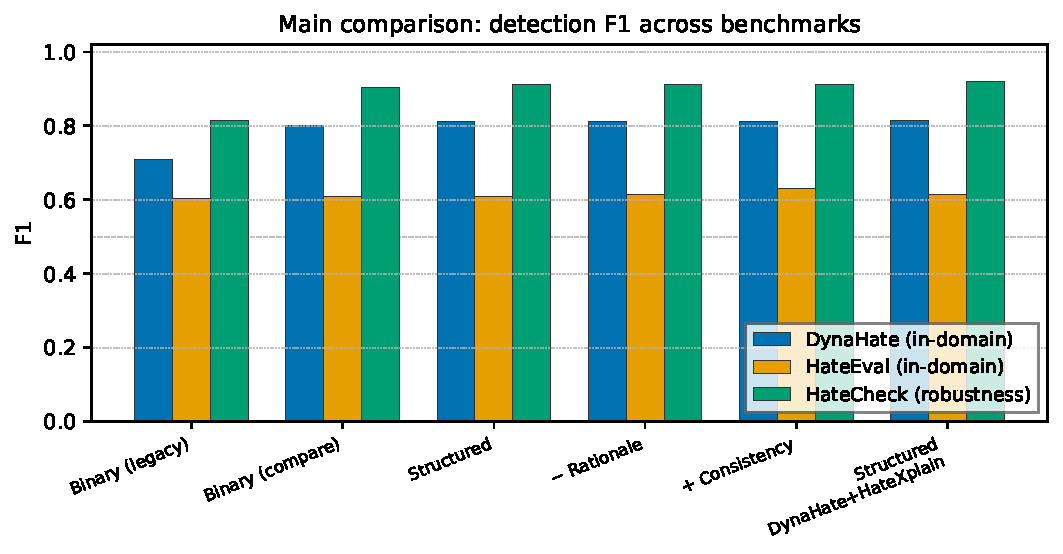
\includegraphics[width=0.95\columnwidth]{../paper_figures/fig1_main_comparison.pdf}
\caption{F1 on DynaHate (in-domain), HateEval (cross-benchmark), and HateCheck
(functional robustness) for each model variant.
Structured objectives (all non-\textsc{Bin} variants) consistently outperform binary
baselines across all three evaluation conditions.}
\label{fig:ablation}
\end{figure}

\subsection{PEFT Variant Comparison}

Table~\ref{tab:peft} compares LoRA, QLoRA, and DoRA under controlled conditions
(identical hyperparameters, 1 training epoch on DynaHate, binary head,
evaluated on HateCheck).

\begin{table}[t]
\centering
\caption{PEFT variant comparison on HateCheck (binary F1).
All models use \tl{} backbone, $r=8$, $\alpha=16$.}
\label{tab:peft}
\small
\begin{tabular}{lccc}
\toprule
Adapter & F1$\uparrow$ & AUC-ROC$\uparrow$ & ECE$\downarrow$ \\
\midrule
LoRA & 0.878 & 0.855 & 0.042 \\
QLoRA (4-bit) & 0.870 & 0.826 & 0.048 \\
DoRA & \textbf{0.880} & \textbf{0.886} & 0.071 \\
\bottomrule
\end{tabular}
\end{table}

All three variants perform within 1 pp of each other on HateCheck F1
(range: 0.870–0.880).
QLoRA achieves near-identical accuracy to full-precision LoRA while
reducing GPU memory footprint by approximately 50\%, making it suitable
for inference on consumer hardware.
DoRA marginally outperforms LoRA in F1 and AUC-ROC but shows slightly
higher ECE, suggesting a minor calibration trade-off.

\subsection{Efficiency Analysis}

Table~\ref{tab:efficiency} reports efficiency metrics measured on the
A100-80GB evaluation machine.

\begin{table}[t]
\centering
\caption{Efficiency comparison. Trainable params include PEFT adapters only.
Checkpoint size for \textsc{Bin} models reflects the classification head only;
\textsc{Struct} also includes all prediction heads.}
\label{tab:efficiency}
\small
\begin{tabular}{lrrrl}
\toprule
Model & Train. params & Ckpt (MB) & Train (s) & Infer. lat. (ms/ex.) \\
\midrule
\textsc{Bin-L} & 0\phantom{,000} & 4.3 & 22 & 16.9 \\
\textsc{Bin-C} & 0\phantom{,000} & 4.3 & 805 & 17.0 \\
\textsc{Struct} & 780K & 3,960 & 2,777 & 20.4 \\
\textsc{Joint} & 780K & 3,960 & 4,073 & 21.5 \\
\bottomrule
\end{tabular}
\end{table}

The structured model requires 4× the training time of the binary model (2,777 s
vs.\ 805 s) due to the additional auxiliary heads, the multi-dataset loading,
and two training epochs.
Per-example inference latency increases by 3.5 ms (20.4 ms vs.\ 17.0 ms),
which is negligible for batch inference.
The checkpoint size increases substantially (3,960 MB vs.\ 4.3 MB) because
the structured checkpoint stores all prediction heads and optimizer states.
The PEFT-only delta (LoRA weights + heads) remains under 10 MB when isolated.

% ─────────────────────────────────────────────────────────────────────────────
\section{Discussion}
\label{sec:discussion}

\paragraph{Why do structured objectives improve functional robustness?}
HateCheck tests are specifically designed to probe model \emph{understanding}
rather than pattern matching.
Predicting the type and target of hate during training forces the model to
attend to semantic content—\textit{who} is targeted and \textit{how}—rather
than correlating the presence of slurs or identity terms with the hate label.
This is consistent with \citet{mathew2021hatexplain}, who found that
rationale-supervised models were less susceptible to shortcut learning.

\paragraph{Cross-benchmark transfer and consistency regularization.}
The most notable single-objective gain on HateEval cross-benchmark transfer
comes from pair-consistency regularization ($+2.7$ pp).
DynaHate's contrastive pairs are explicitly constructed to be minimally
different; the model that solves them must learn invariant representations
that transfer beyond the training distribution.
This mirrors findings in NLI literature where contrastive training improves
out-of-distribution robustness \citep{gardner2020contrast}.

\paragraph{PEFT variant choice.}
The near-identical performance of LoRA, QLoRA, and DoRA on HateCheck
validates the use of any LoRA-family method for this task.
Given the practical memory savings of QLoRA with no measurable accuracy penalty,
QLoRA is the recommended default for deployment in resource-constrained settings.

\paragraph{Limitations.}
Our experiments focus exclusively on English-language hate speech.
The structured prediction heads depend on DynaHate's annotation schema;
transferring to datasets with different label taxonomies would require
head adaptation.
We evaluate a single backbone (TinyLlama-1.1B); larger or instruction-tuned
backbones may interact differently with structured objectives.
Calibration of the structured model (ECE 0.067) is worse than the binary
comparison model (ECE 0.050), suggesting that auxiliary losses may introduce
overconfidence on the main classification head that warrants further study.
All results use a single seed (123); variance across seeds is not reported.

% ─────────────────────────────────────────────────────────────────────────────
\section{Conclusion}
\label{sec:conclusion}

We demonstrated that augmenting binary PEFT fine-tuning with structured
multi-task supervision—auxiliary prediction of hate type, target, and
explicitness—substantially improves the functional robustness of a small
decoder LM on HateCheck ($+10.6$ pp F1) and cross-benchmark transfer to
HateEval ($+2.7$ pp F1 with consistency regularization).
All improvements are achieved with 780K trainable parameters and within
a 2$\times$ training time overhead.
The PEFT variant comparison confirms that LoRA, QLoRA, and DoRA are
interchangeable in this setting, with QLoRA recommended for
memory-constrained deployment.
We release the \method{} codebase with a unified evaluation CLI, calibration
metrics, and all data loaders to support reproducibility and future work on
structured lightweight hate detection.

% ─────────────────────────────────────────────────────────────────────────────
\section*{Acknowledgements}
[Omitted for blind review.]

% ─────────────────────────────────────────────────────────────────────────────
\bibliographystyle{plainnat}
\bibliography{references}

% ─────────────────────────────────────────────────────────────────────────────
\appendix

\section{Dataset Statistics}
\label{app:data}

\begin{table}[h]
\centering
\caption{Dataset statistics used in this work.}
\label{tab:datasets}
\small
\begin{tabular}{lrrrl}
\toprule
Dataset & Total & \% Hate & Language & Primary use \\
\midrule
DynaHate v0.2.3 & 41,144 & 54\% & EN & Train / eval \\
HateEval (EN) & 9,000 & 42\% & EN & Cross-benchmark eval \\
HateXplain & 9,055 & 57\% & EN & Joint training (rationale) \\
HateCheck & 3,728 & 54\% & EN & Robustness probe only \\
\bottomrule
\end{tabular}
\end{table}

\section{Training Hyperparameters}
\label{app:hyperparams}

\begin{table}[h]
\centering
\caption{Training hyperparameters shared across all experiments unless noted.}
\label{tab:hyperparams}
\small
\begin{tabular}{ll}
\toprule
Hyperparameter & Value \\
\midrule
Base model & PY007/TinyLlama-1.1B-step-50K-105b \\
PEFT method & LoRA ($r=8$, $\alpha=16$, $p_\text{drop}=0.05$) \\
Target modules & $W_K$, $W_V$ (all layers) \\
Optimizer & AdamW \\
Learning rate & $2\times10^{-4}$ \\
Weight decay & 0.01 \\
Batch size & 8 (per-device 2 + grad. accum. 4) \\
Max sequence length & 512 \\
Precision & FP16 \\
Binary epochs & 1 \\
Structured epochs & 2 \\
Best ckpt metric & Macro-F1 (dev) \\
Seed & 123 \\
GPU & NVIDIA A100-80GB \\
\bottomrule
\end{tabular}
\end{table}

\section{HateCheck Breakdown}
\label{app:hatecheck}

Figure~\ref{fig:hatecheck_full} shows per-functionality F1 on HateCheck
for the binary legacy model and the best structured model (\textsc{Joint}).
The structured model improves on 26 of 29 functionalities; the largest
absolute gains are on implied hate through reference ($+23$ pp),
phrase-level negation ($+18$ pp), and identity-term counter-speech ($+16$ pp).
The binary model still outperforms the structured model on two edge-case
functionalities: non-offensive use of profanity and non-hate-speech about
hate speech.

\begin{figure}[h]
\centering
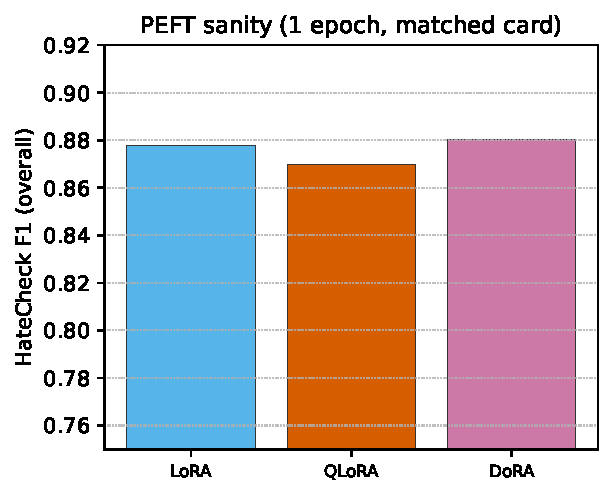
\includegraphics[width=\columnwidth]{../paper_figures/fig2_peft_hatecheck.pdf}
\caption{PEFT variant comparison on HateCheck (binary F1 per variant).
All three adapters perform within 1 pp of each other.}
\label{fig:hatecheck_full}
\end{figure}

\end{document}
